\chapter{Background}

Questo capitolo mira a fornire tutte le informazioni necessarie per comprendere il lavoro svolto e le tecnologie utilizzate.  Dapprima vedremo cosa significa bug o errore e perché è rilevante risolverli. Vedremo poi quali sono i principali strumenti utilizzati per rilevare bug, come Sanitizers e Fuzzing e i benefici della loro implementazione simultanea. 

\section{Bug e Vulnerabilità}

Un bug è un difetto in un software che porta ad un risultato inaspettato. Errori nei software sono dovuti ad errori umani nel codice, compilatore o sistema runtime \cite{ref3}. Questi portano il programma in uno stato non voluto e ne causano possibilmente il blocco. Solo nel caso in cui il bug potrebbe permettere ad un attaccante la compromissione di Confidenzialità, Integrità o Disponibilità si parla allora di vulnerabilità \cite{ref1}.

Una vulnerabilità è quindi una debolezza del sistema che permette ad un attaccante di sfruttare un bug. Richiede 3 componenti principali: 
\begin{enumerate}
    \item un sistema suscettibile al difetto;
    \item un avversario con accesso al difetto;
    \item un avversario che abbia le capacità di sfruttare il difetto \cite{ref1}. 
\end{enumerate}

La sicurezza di un sistema software è disciplinata da un insieme di principi fondamentali. Quando questi principi sono rispettati, il software può essere considerato sicuro. Tra le principali dimensioni della sicurezza informatica si distinguono la Memory Safety e la Type Safety.

La Memory Safety garantisce che ogni puntatore faccia riferimento esclusivamente a celle di memoria valide e correttamente allocate \cite{ref4}. La Type Safety, invece, assicura che gli oggetti vengano utilizzati in conformità al loro tipo, rispettando la gerarchia dei tipi e le conversioni (cast) corrette durante l’esecuzione del programma \cite{ref5}.
La presenza di bug nel codice può compromettere la memory o type safety, esponendo il programma a vulnerabilità sfruttabili per modificare il suo stato di runtime. In tali casi, un attaccante potrebbe eseguire operazioni malevole. Quando un programma non segue più controlli definiti e flussi di dati corretti, si può parlare di una weird machine \cite{ref2}. 
Il rispetto della memory e type safety consente di prevenire difetti a basso livello, limitando l’esposizione del software a vulnerabilità logiche specifiche.
Va inoltre sottolineato che i requisiti di sicurezza non sono direttamente testabili. Il testing consente di individuare la presenza di errori, ma non la loro completa assenza. L’obiettivo del testing, in questo contesto, è verificare se durante l’esecuzione vengano rispettate le proprietà di memory e type safety \cite{ref6}.

Nonostante ciò, il Testing resta una componente essenziale nel ciclo di vita di un software, ad ogni aggiornamento o ulteriore implementazione di funzionalità deve seguire un rigido regime di testing. Il testing si divide principalmente in due categorie: Statico e Dinamico.
Il testing Statico si riferisce a tutte quelle tecniche capaci di rilevare errori senza eseguire il codice. Tra questi troviamo symbolic execution. Il testing dinamico invece esegue il programma e rileva errori osservando il comportamento durante l’esecuzione. Nel lavoro di questa tesi sono stati utilizzati strumenti di testing dinamico, sanitizers e fuzzers. L’idea alla base è combinare le molteplici esecuzioni del fuzzing che permette di esplorare più percorsi possibili ai controlli aggiuntivi imposti dai sanitizer che validare queste esecuzioni. 

\section{Sanitizers}

Esistono diversi tipi di tecniche di testing: le più comuni si limitano a rilevare bug tramite asserzioni, segmentation faults o eccezioni che causano la terminazione del programma. Tuttavia, queste tecniche non sempre riescono a individuare errori più sottili, che non portano immediatamente a un crash ma possono comunque compromettere la correttezza della computazione \cite{ref1}.

Per affrontare questi casi, sono stati sviluppati strumenti noti come Sanitizers, i quali inseriscono, già in fase di compilazione, un codice di strumentazione che controlla e valida il comportamento del programma durante l’esecuzione. Ogni sanitizer è specializzato nell’individuare una specifica classe di bug (o poche classi affini), come ad esempio buffer overflows, utilizzo di valori non inizializzati o differenziazione di indirizzi non validi. In pochi anni, questi strumenti sono diventati essenziali nell’identificare vulnerabilità \cite{ref19}. Il primo strumento di questo tipo fu l’AddressSanitizer (ASan), introdotto da Google nel 2012, progettato per rilevare errori di memoria come use-after-free e accessi fuori dai limiti \cite{ref7}, \cite{ref18}. 

\begin{figure}[htbp]        
  \centering               
  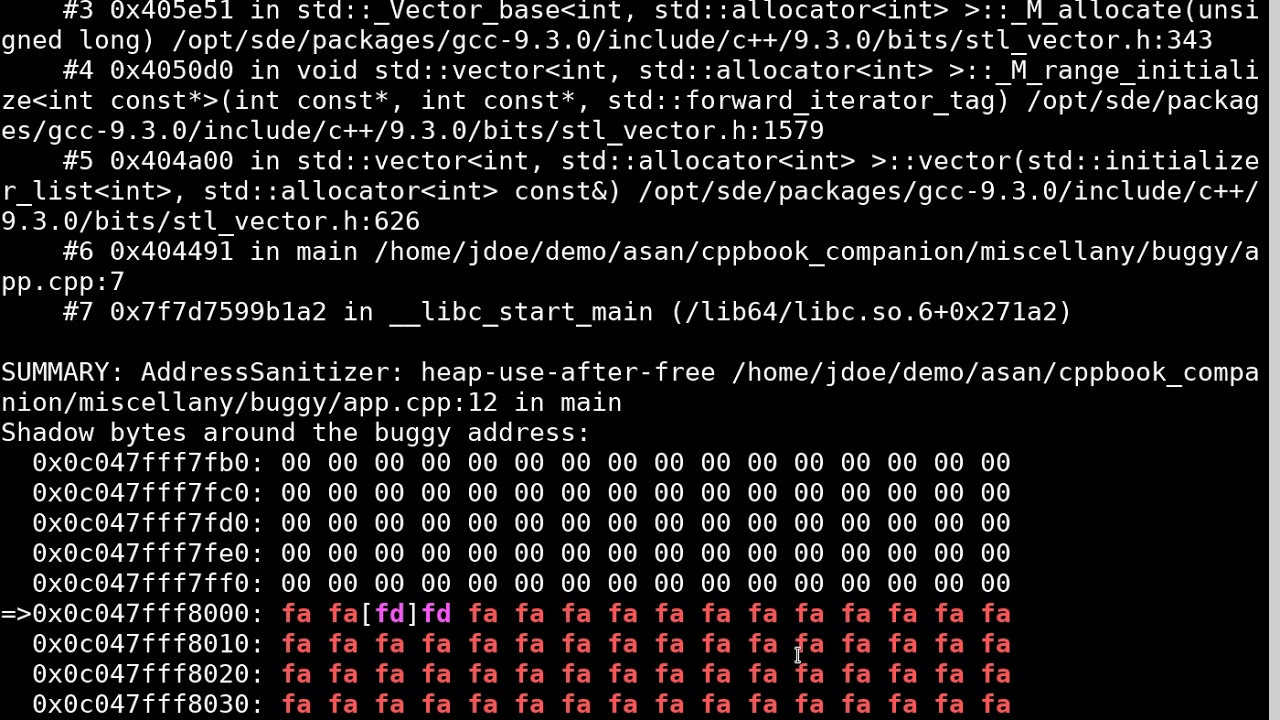
\includegraphics[width=0.7\textwidth]{immagini/asan.jpg}  
  \caption{Esempio di utilizzo di ASan}  
  \label{fig:asan}      
\end{figure}

\subsection{MSan}

In questo progetto di tesi ci siamo concentrati sull’individuazione dei bug noti come Use of Uninitialized Memory (UUM),  ossia l’utilizzo di memoria non inizializzata durante l’esecuzione di un programma \cite{ref13}. Il sanitizer più diffuso per questa categoria di errori è il MemorySanitizer (MSan), sviluppato da Google nel 2015 \cite{ref8}.

Questo è un detector di memory read per C/C++ che aiuta gli sviluppatori a trovare e aggiustare errori di tipo UUM, considerati solitamente difficili da trovare in quanto non occorrono in ogni esecuzione e possono essere triggerati da una qualunque operazione del programma. I linguaggi C/C++ in particolare lasciano allo sviluppatore il compito di allocare, utilizzare e liberare correttamente ogni cella di memoria acceduta dal  programma - sono definite per questo motivo memory-unsafe \cite{ref5}. Questo tipo di vulnerabilità non possono essere sfruttate solo per alterare il flusso di esecuzione del programma ma anche per rilevare informazioni sullo stato interno del programma e contenuti dello stack/heap \cite{ref16}. 

Un bug di tipo UUM si origina solitamente quando viene utilizzata una variabile o un buffer prima della sua inizializzazione. Questo risulta essere  pericoloso poiché le variabili locali non inizializzate contengono valori casuali (spesso derivati da utilizzi precedenti della memoria) e l’utilizzo di queste variabili porta ad un comportamento indefinito del programma \cite{ref9}.

MSan adotta un approccio compiler-based, in quanto inserisce nel programma, in fase di compilazione, istruzioni aggiuntive per tracciare lo stato di inizializzazione di ogni cella di memoria. Il suo funzionamento si fonda sul concetto di shadow memory, una memoria parallela che mantiene le informazioni sullo stato della memoria principale \cite{ref8}. Ogni operazione di scrittura aggiorna la shadow memory, mentre ogni operazione di lettura è accompagnata da un controllo che permette di intercettare l’uso di valori non inizializzati \cite{ref3}.

Un aspetto complesso di questo approccio è che non tutti i pattern rilevati come potenzialmente pericolosi corrispondono a veri bug. Alcune istruzioni apparentemente in conflitto con i principi di memory safety sono in realtà introdotte dal compilatore per motivi di ottimizzazione \cite{12}. Per ridurre i falsi positivi, MSan concentra quindi le verifiche su eventi semanticamente rilevanti per l’esecuzione, come:
\begin{itemize}
    \item la valutazione di una branch condition;
    \item la dereferenziazione di un puntatore;
    \item il passaggio di dati a una system call o a una chiamata di libreria sensibile.
\end{itemize}

Per garantire la correttezza del tracciamento, i sanitizer per UUM devono modellare il flusso dei dati attraverso le diverse istruzioni, operazione nota come shadow propagation. Questo riduce i falsi positivi (ad esempio nei casi di copia di memoria non inizializzata), ma introduce un overhead significativo a runtime. Inoltre, uno dei principali limiti di MSan consiste nella necessità di ricompilare tutte le librerie con la strumentazione: in assenza di tale ricompilazione, il numero di falsi positivi cresce sensibilmente \cite{ref12}.

\subsection{QMSan}

Questo lavoro di tesi ha utilizzato lo strumento QMSan, un sanitizer che riprende i concetti fondamentali di MSan e supera alcune limitazioni strutturali. QMSan utilizza QEMU User Emulation, a differenza di MSan, quindi non richiede la ricompilazione completa delle librerie né il codice sorgente. Questo lo rende anche applicabile immediatamente a software binari di terze parti o a librerie che non hanno il sorgente \cite{ref12}.

Mentre MSan monitora lo stato di inizializzazione solo per gli oggetti che osservano l'allocazione o la deallocazione, QMSan sfrutta una tecnica più semplice ed efficace: considera la memoria come non inizializzata di default; lo stato viene aggiornato solo dopo le operazioni di scrittura. 

Questo consente di mantenere un tracciamento coerente a livello binario, riducendo le ambiguità tipiche dell’approccio compiler-based. Pertanto, è possibile mantenere un tracciamento coerente a livello binario, riducendo le ambiguità tipiche dell'approccio basato sul compilatore.

Il suo design multi-layer opportunistico è un'innovazione significativa di QMSan. Inizialmente, il sistema utilizza un detector leggero che cerca anomalie nelle operazioni di load and store. Il programma viene rieseguito utilizzando un detector accurato basato su shadow propagation completa quando viene scoperto un bug sospetto. Se l'anomalia si dimostra un falso positivo, viene registrata e ignorata nelle esecuzioni successive per evitare di ripetere controlli ridondanti.

Questa architettura consente a QMSan di mantenere un buon compromesso tra accuratezza e performance, con un overhead significativamente inferiore rispetto a Memcheck e altri strumenti binari. La sua compatibilità universale lo rende utilizzabile con qualsiasi binario, indipendentemente dalla ricompilazione o dal supporto del compilatore. In questo senso, QMSan è una soluzione più pratica e flessibile rispetto a MSan, specialmente quando si tratta di fuzzing di software di terze parti o proprietario.

\subsection{Valgrind}

Valgrind è un framework di analisi dinamica popolare per il debugging di applicazioni scritte in linguaggi a basso livello come C++ e C. La capacità di rilevare errori di memoria come accessi fuori dai limiti, utilizzo di memoria non inizializzata e perdite di memoria sono tra le sue caratteristiche principali \cite{ref14}, \cite{ref15}. Tuttavia, la capacità di creare uno stack trace preciso e affidabile in caso di crash è tra le caratteristiche più importanti del debugging avanzato. Quando un programma si arresta in modo anomalo, identificare esattamente dove si è verificato l'errore è fondamentale per comprendere la causa del problema e creare una correzione efficace.

Valgrind monitora l'esecuzione del programma in un ambiente virtualizzato e traccia ogni operazione di memoria. Questa modalità consente allo strumento di mantenere informazioni accurate sul contesto di ogni istruzione eseguita, inclusi i registri della CPU e i puntatori di stack. Ciò evita le ambiguità che si verificano spesso durante un crash normale del sistema. Ciò significa che Valgrind può fornire un backtrace accurato e coerente anche in presenza di buffer overflow o corruzioni di memoria, mostrando i parametri passati e gli indirizzi di ritorno della sequenza di chiamate di funzione che ha causato il crash.

In contesti di testing automatizzato e di fuzzing, dove i crash possono verificarsi in modo imprevisto e su percorsi di codice poco esplorati, Valgrind è uno strumento molto utile. Questo perché ha la capacità di creare uno stack affidabile. In particolare, per quanto riguarda i valori non definiti \cite{ref10}. Lo stack trace creato da Valgrind non solo consente di identificare rapidamente il punto di origine dell'errore, ma fornisce anche informazioni utili per ottimizzare le strategie di fuzzing o per creare nuovi sanitizer nei workflow sperimentali. In particolare, Valgrind garantisce una tracciabilità completa, rendendo possibile la riproduzione del bug e la verifica della sua natura in modo affidabile. Ciò lo distingue dai crash comuni, in cui lo stack può essere corrotto o parzialmente leggibile.

\section{Fuzzing}

Il fuzzing è una delle tecniche di testing automatico più diffuse grazie alla capacità di rilevare problemi critici. Questa tecnica consiste nel sollecitare sistematicamente un programma con una serie di input casuali o inaspettati per verificare che non avvengano crash, eccezioni o terminazioni anomale \cite{ref17}, \cite{ref20}.  Questo strumento è particolarmente efficace, quando comparato a tool come angr (utilizzato per la symbolic execution), AFL (fuzzing tool che vedremo successivamente) è riuscito a trovare più bug in un periodo di 24 ore \cite{ref29}.

Gli input nel fuzzing sono generati automaticamente e spesso includono elementi di randomicità; particolare attenzione è posta ai casi limite (edge cases). Un fuzzer è lo strumento che implementa il processo di fuzzing: esegue un ciclo automatizzato guidato da feedback e mantiene una coda (corpus) di test case. Il funzionamento tipico di un fuzzer può essere descritto come segue:
\begin{enumerate}
    \item si inizializza la coda con un insieme di input detto corpus;
    \item si generano nuovi input mutando quelli presenti nella coda o generandone di nuovi;
    \item si esegue il programma con gli input prodotti;
    \item si osservano informazioni di esecuzione (es. crash, code coverage, asserzioni) e si raccoglie feedbacksi mantengono nella coda gli input ritenuti interessanti per successive mutazioni e analisi \cite{ref1}.
\end{enumerate}

\begin{figure}[htbp]        
  \centering               
  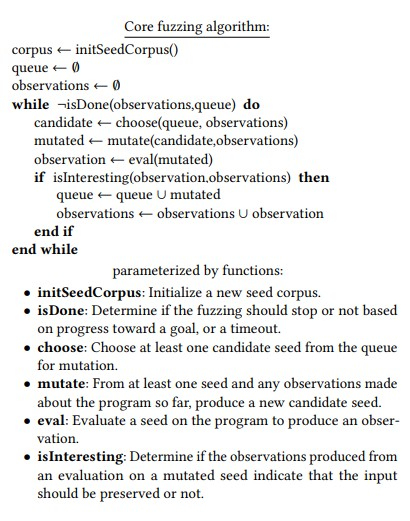
\includegraphics[width=0.6\textwidth]{immagini/fuzzing.jpg}  
  \caption{Fuzzing come schema algoritmico \cite{ref21}}  
  \label{fig:fuzzing}      
\end{figure}

In una prima fase, il fuzzer organizza la coda con i seeds: un insieme di input validi o semi-validi. Questi permettono al fuzzer di esplorare percorsi realistici, superando i controlli basilari di validazione e penetrando più a fondo nella logica del programma. Anche un singolo seed efficace può garantire una copertura significativa. In assenza di seeds, il fuzzer tenderà a generare molti input che causeranno la terminazione immediata del programma, fino a quando non sarà in grado di apprendere come superare autonomamente i controlli iniziali. Spesso vengono utilizzati test cases provenienti da fonti esterne, forniti come input al programma per osservare il suo comportamento.

Il mutatore rappresenta una delle componenti principali del fuzzer: esso genera nuovi input a partire da uno o più elementi presenti nella coda. In questo modo è possibile ottenere input non solo nuovi, ma anche diversificati, aumentando l’efficacia del corpus che potrà essere sfruttato in sessioni future. L’obiettivo di un buon fuzzer è produrre input sufficientemente validi da essere accettati, ma al tempo stesso abbastanza anomali da poter innescare condizioni limite. 

In letteratura si distinguono due principali approcci: mutation-based e generation-based.

I mutation-based fuzzers richiedono un set iniziale di seeds; a partire da questi applicano un insieme di trasformazioni come bit flip, inserimento o rimozione di byte, operazioni aritmetiche e combinazioni tra input differenti. Tali strumenti integrano strategie sia deterministiche che non deterministiche per selezionare e schedulare le mutazioni a ogni tentativo di generazione.

I generation-based fuzzers, invece, non necessitano di seeds iniziali poiché sono in grado di creare input ex novo basandosi su meccanismi di randomicità. Tuttavia, questo approccio richiede generalmente più tempo per generare input di qualità e per ottenere risultati comparabili a quelli basati su mutazioni.

Un ulteriore aspetto cruciale riguarda le performance: l’obiettivo è ottimizzare il numero di esecuzioni ripetute e monitorare come l’input raggiunga il codice da testare. Spesso, per facilitare questa attività, gli sviluppatori implementano un harness, ossia un frammento di codice progettato per leggere i dati forniti dal fuzzer e invocare le porzioni di codice da testare.

Infine, un meccanismo di feedback accurato è essenziale per garantire l’efficacia di un fuzzer. Per ciascun test case eseguito, il fuzzer raccoglie un profilo di esecuzione e lo confronta con le esecuzioni precedenti, in modo da identificare input che conducano a percorsi nuovi o interessanti del programma. I fuzzer possono essere accompagnati da diverse tecniche di analisi finalizzate ad aumentarne l’efficienza e l’efficacia. Si distinguono principalmente tre approcci: 
\begin{itemize}
    \item Black-box fuzzing: in questo caso il fuzzer non ha alcuna conoscenza della struttura interna del programma. È particolarmente efficace nell’individuare i cosiddetti bug di superficie, ossia errori che non richiedono un’esplorazione profonda del codice per essere rilevati. Questo approccio si caratterizza per semplicità, velocità e scalabilità, ma non garantisce necessariamente la copertura di percorsi complessi del programma;
    \item White-box fuzzing: al contrario, il fuzzer dispone di informazioni dettagliate sulla struttura interna del programma e genera input accuratamente progettati per esplorare il maggior numero possibile di percorsi. Questo metodo consente di individuare vulnerabilità collocate in profondità, ma comporta costi elevati in termini di tempo e risorse computazionali a causa delle analisi strutturali richieste. Inoltre, non sempre riesce a rilevare errori che un approccio più esplorativo avrebbe potuto scoprire;
    \item Grey-box fuzzing : in questo modello il fuzzer dispone di alcune informazioni parziali sul programma, senza tuttavia conoscerne completamente la struttura interna. Tale compromesso consente di guidare l’esplorazione verso percorsi rilevanti, mantenendo al tempo stesso un buon livello di indipendenza e flessibilità nell’esecuzione \cite{ref22}.
\end{itemize}

I grey-box fuzzers sono anche noti come coverage-guided fuzzers, in quanto l’esplorazione del programma in fase di test viene regolata da meccanismi di coverage feedback. Durante l’esecuzione, infatti, viene mantenuta una coverage map: una rappresentazione che registra le porzioni di codice raggiunte dagli input. Ogni volta che viene eseguita una nuova sezione del programma, la mappa viene aggiornata di conseguenza \cite{ref23}.

Questo meccanismo permette di identificare rapidamente quali input conducono a percorsi di esecuzione nuovi o inesplorati. Gli input ritenuti “interessanti” vengono conservati nella coda del fuzzer per ulteriori mutazioni, in modo da ampliare progressivamente la copertura del programma e aumentare le probabilità di individuare bug profondi o edge cases.

In generale, misurare le performance di un fuzzer risulta piuttosto difficile, bisogna tenere in considerazione che:
\begin{itemize}
    \item esiste la necessità di eseguire molteplici campagne - abbastanza per tenere conto della variazione della performance tra un run ed il successivo;
    \item molte analisi misurano la performance di un fuzzer contando i crashes unici piuttosto che i bug distinti, questo può portare a sovrastimare il numero di bug;
    \item i seed giocano un ruolo importante all'interno del fuzzer, un cambiamento di seed tra una campagna e l'altra può variare sostanzialmente la performance \cite{ref21}. 
\end{itemize}

\subsection{AFL++}

Il fuzzer più popolare, e quello che è stato utilizzato nello svolgimento di questo tirocinio è American Fuzzy Loop ++ (AFL++), uno sviluppo dell’omonimo AFL \cite{ref11}, \cite{ref24}.Questo è un fuzzer di tipo coverage-guided. 

La metrica principale per la performance di un fuzzer è data dai crashes, ma altre caratteristiche da prendere in considerazione sono:
\begin{itemize}
    \item throughput (exec/sec): test cases completati nell’unità di tempo;
    \item queue size (“total paths”): test cases distinti generati;
    \item coverage: numero di edges coperti dal programma.
\end{itemize}

\begin{figure}[htbp]        
  \centering               
  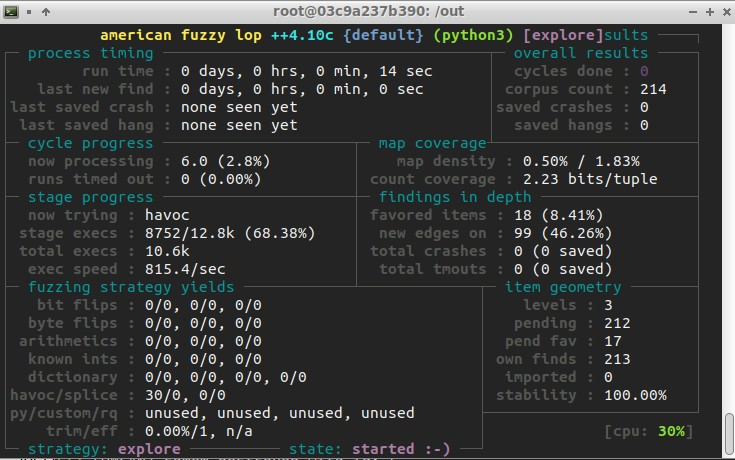
\includegraphics[width=0.8\textwidth]{immagini/AFL++.jpg}  
  \caption{schermata di AFL++}  
  \label{fig:afl++}      
\end{figure}

I primi due sono calcolati da AFL++,  il terzo viene derivato processando la coda. 
Throughput è particolarmente importante, maggiori sono le esecuzioni maggiori sono le probabilità di trovare un bug. Talvolta gli input rigettati possono condizionare questa metrica in quanto sono considerate esecuzioni particolarmente veloci. 
Bisogna poi tenere conto della lunghezza della coda, infatti, una lunghezza troppo corta può significare che l’esplorazione è troppo superficiale mentre una coda troppo lunga non darà abbastanza tempo al fuzzer per mutare tutti gli input interessanti. 
Un’altra metrica è la code coverage che ci descrive quanto il programma è stato esplorato e quali parti. Maggiore questa è, più parti del programma abbiamo esplorato. 

AFL ci fornisce come output una serie di file con le statistiche relatve alla campagna e i relativi log ma anche una serie di cartelle:
\begin{itemize}
    \item crashes/: vengono conservati i test cases che producono crashes per permettere di riprodurli successivamente ed analizzarli;
    \item hangs/: input che si bloccano o restano indefinitivamente bloccati in un loop;
    \item queue/: conserva gli inpt che si sono dimostrati capaci di esplorare grandi o nuove parti de programma.
\end{itemize}
Per quanto riguarda la coda mantiene dinamicamente un insieme di input di test-cases non ridonanti che permettono di esplorare tutti gli edges (coperti fino a quel momento) della mappa. 

\subsection{Fuzzer Test Suite}

I Fuzzer Test Suite (FTS) sono un insieme di benchmark sviluppate Google, create per testare sistematicamente l’efficacia e le prestazioni dei fuzzer. Questa infatti raccoglie programmi reali che in passato hanno avuto serie vulnerabilità; queste vulnerabilità sono state poi documentate, diventando così un riferimento affidabile per misurare la capacità dei fuzzer di individuare bug.  Per questo motivo FTS è ampiamente utilizzato nell’ambito della ricerca accademica e nello sviluppo di nuovi fuzzers e sanitizers, mette infatti a disposizione un ambiente di testing comunque e riproducibile.

Nell’ambito di questo tirocinio, l’FTS è stato impiegato per verificare la validità del mio setup sperimentale.  

\subsection{OSS-Fuzz}

Oss-Fuzz è un servizio di fuzzing continuo fornito da Google per progetti di tipo open-source. Il suo lavoro è quello di ottimizzare le esecuzioni di molteplici fuzzer su build strumentate e coordinare la raccolta, deduplicazione e segnalazione dei crashes. Esegue quindi testing su larga scala ed invia report riproducibili e tracciabili ai manutentori dei progetti. Questo approccio permette di scoprire vulnerabilità reali in modo proattivo, migliorando la qualità del software e fornendo un ambiente di testing continuo e standardizzato. 

Nasce nel 2016, a seguito della scoperta della vulnerabilità Heartbleed in OpenSSL, uno dei programmi più popolari per la crittazione di traffico web e avendo quindi il potenziale di coinvolgere tutti gli utenti di Internet \cite{ref30}. Questo bug si rivelò essere un semplice caso di buffer overflow. Google crea OSS-Fuzz per riempire questo vuoto, dalla sua implementazione è diventato un servizio critico per la comunità open-sorce, espandendo il proprio reach oltre ai linguaggi di C/C++ ed includendone altri come Go, Rust e Python. Nel corso degli anni è riuscto ad identificare e correggere oltre 10.000 vulnerabilità.

\begin{figure}[htbp]        
  \centering               
  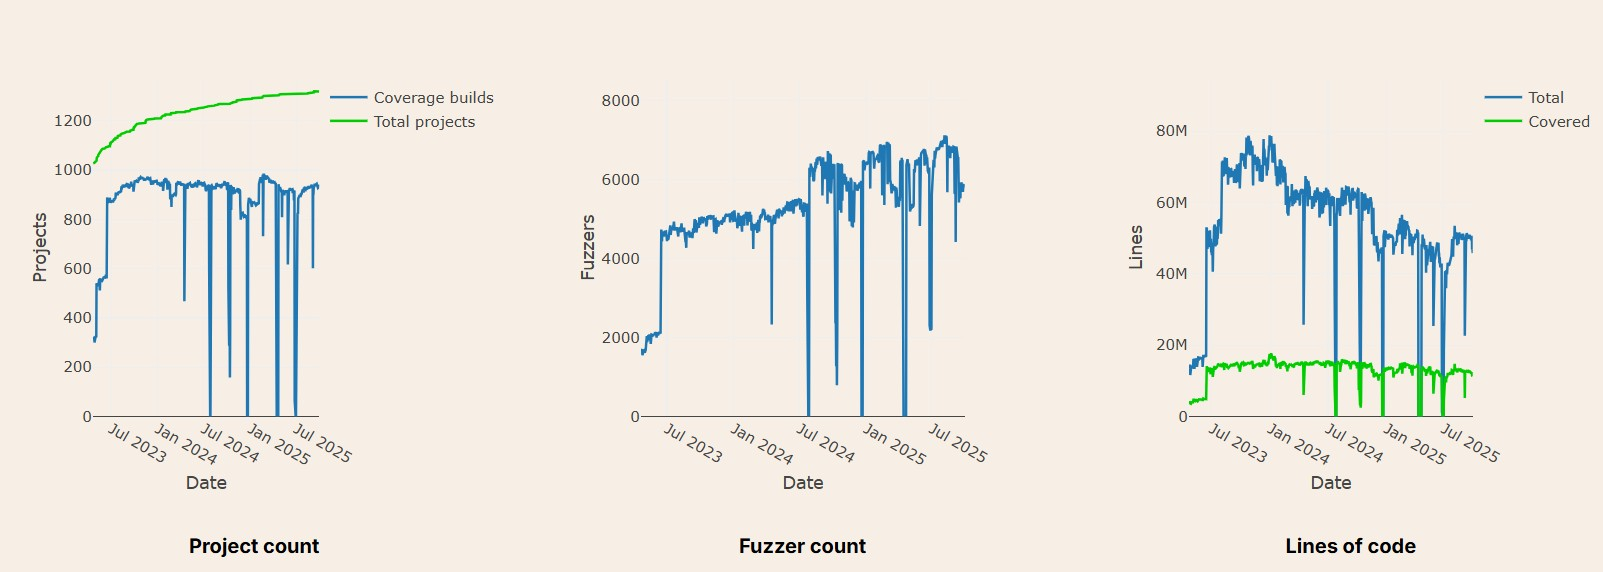
\includegraphics[width=0.7\textwidth]{immagini/oss-fuzz_stats.jpg}  
  \caption{Statistiche relative ad OSS-Fuzz \cite{ref31}}  
  \label{fig:oss-fuzz_stats}      
\end{figure}

Il processo di OSS-Fuzz si struttura nel seguente modo:
\begin{enumerate}
  \item Inizialmente, lo sviluppatore crea i fuzz target, che sono piccoli programmi che funzionano con le librerie del progetto e ricevono sequenze di dati modificate o create casualmente. I file di configurazione di build vengono quindi definiti e inviati nella repository ufficiale di OSS-Fuzz;
  \item A questo punto, il servizio di Cloud Build interviene sincronizzando il codice sorgente del progetto upstream e compilandolo con i fuzzer, creando così i binari eseguibili. Un bucket di Google Cloud Storage (GCS), che funge da archivio centralizzato, contiene tali oggetti;
  \item ClusterFuzz, il motore che esegue il fuzzing su larga scala, scarica e esegue i fuzzer in modo distribuito. Questo apre automaticamente un ticket all'interno dell'issue tracker Monorail in caso di crash o comportamenti anomali, allegando log, input di riproduzione e stack trace utili all'analisi. Inoltre, il sistema controlla regolarmente se i bug segnalati persistono anche dopo le correzioni;
  \item Sheriffbot interviene anche per rispettare le scadenze e risolvere le vulnerabilità tempestivamente. Successivamente alle segnalazioni, lo sviluppatore può correggere i bug e assegnare le patch al progetto originario. Il ciclo ricomincia automaticamente, consentendo di verificare l'efficacia della riparazione e di mantenere il software costantemente testato;
\end{enumerate}

In questo modo, OSS-Fuzz implementa un modello di continuous fuzzing, integrando compilazione, testing e gestione dei bug in un processo completamente automatizzato, il che riduce notevolmente il rischio di vulnerabilità non individuate.

\begin{figure}[htbp]        
  \centering               
  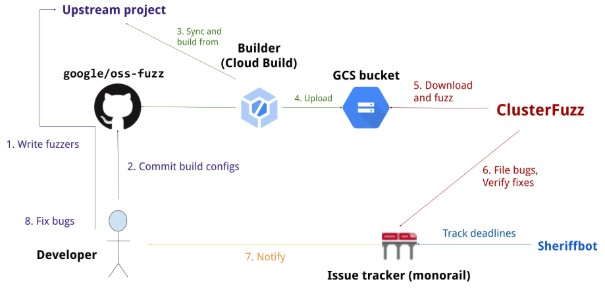
\includegraphics[width=0.7\textwidth]{immagini/oss-fuzz.jpg}  
  \caption{Come funziona OSS-Fuzz}  
  \label{fig:oss-fuzz}      
\end{figure}

Nel contesto di questo tirocinio, alcuni programmi di OSS-Fuzz sono stati testati attraverso una combinazione di fuzzing e l’utilizzo del sanitizer QMSan con lo scopo di individuare UUM bug tralasciati dal sistema automatico di reporting di OSS-Fuzz.
